%%%%%%%%%%%%%%%%%%%%%%%%%%%%%%%%%%%%%%%%%
% The Legrand Orange Book
% LaTeX Template
% Version 2.2 (30/3/17)
%
% This template has been downloaded from:
% http://www.LaTeXTemplates.com
%
% Original author:
% Mathias Legrand (legrand.mathias@gmail.com) with modifications by:
% Vel (vel@latextemplates.com)
%
% License:
% CC BY-NC-SA 3.0 (http://creativecommons.org/licenses/by-nc-sa/3.0/)
%
% Compiling this template:
% This template uses biber for its bibliography and makeindex for its index.
% When you first open the template, compile it from the command line with the
% commands below to make sure your LaTeX distribution is configured correctly:
%
% 1) pdflatex main
% 2) makeindex main.idx -s StyleInd.ist
% 3) biber main
% 4) pdflatex main x 2
%
% After this, when you wish to update the bibliography/index use the appropriate
% command above and make sure to compile with pdflatex several times
% afterwards to propagate your changes to the document.
%
% This template also uses a number of packages which may need to be
% updated to the newest versions for the template to compile. It is strongly
% recommended you update your LaTeX distribution if you have any
% compilation errors.
%
% Important note:
% Chapter heading images should have a 2:1 width:height ratio,
% e.g. 920px width and 460px height.
%
%%%%%%%%%%%%%%%%%%%%%%%%%%%%%%%%%%%%%%%%%

%----------------------------------------------------------------------------------------
%	PACKAGES AND OTHER DOCUMENT CONFIGURATIONS
%----------------------------------------------------------------------------------------

\documentclass[11pt]{book} % Default font size and left-justified equations

%----------------------------------------------------------------------------------------

\input{structure} % Insert the commands.tex file which contains the majority of the structure behind the template

\begin{document}

%----------------------------------------------------------------------------------------
%	TITLE PAGE
%----------------------------------------------------------------------------------------

\begingroup
\thispagestyle{empty}
\begin{tikzpicture}[remember picture,overlay]
\node[inner sep=0pt] (background) at (current page.center) {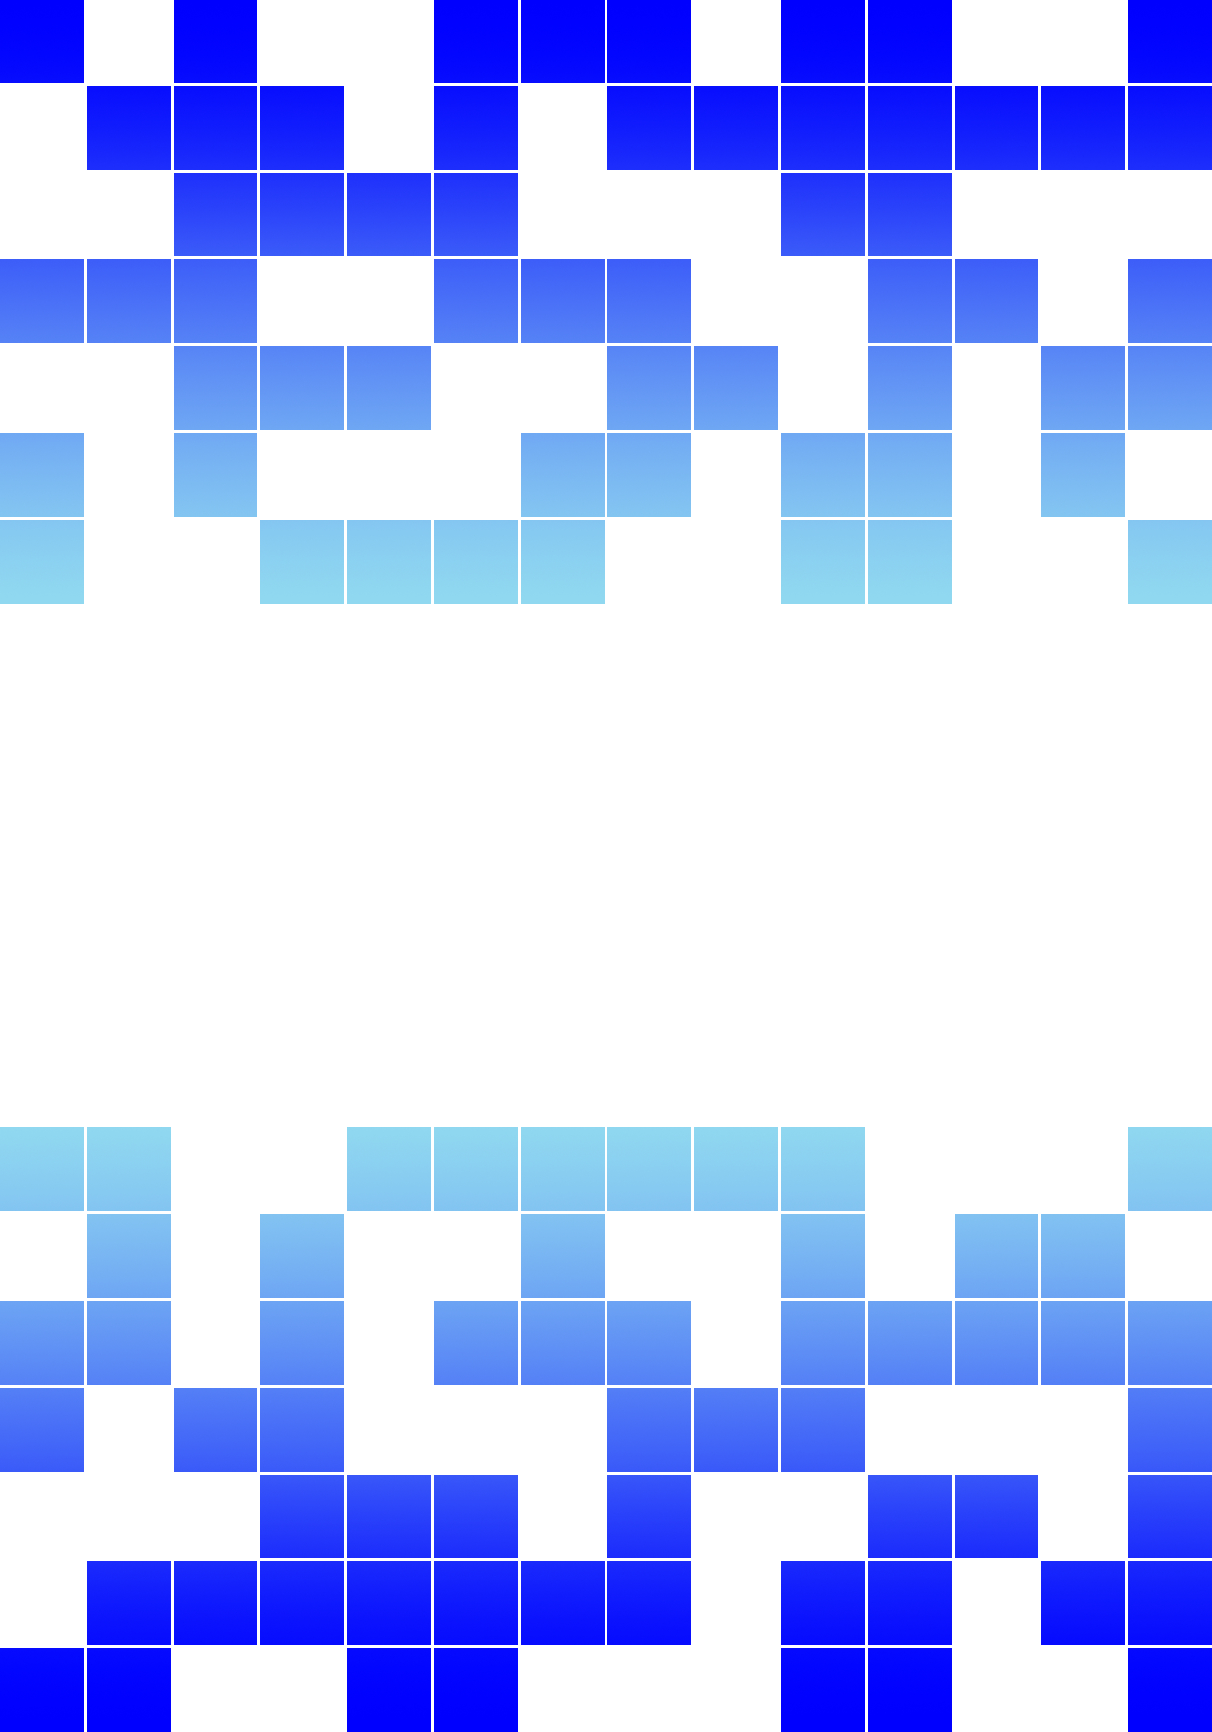
\includegraphics[width=\paperwidth]{background}};
\draw (current page.center) node [fill=steelblue!30!white,fill opacity=0.6,text opacity=1,inner sep=1cm]{\Huge\centering\bfseries\sffamily\parbox[c][][t]{\paperwidth}{\centering Naines blanches, étoiles à neutrons et étoiles étranges\\[15pt] % Book title
{\Large Les états exotiques de la matière dans les corps hyperdenses}\\[20pt] % Subtitle
{\huge Nicolas BELLEMONT et Théo TURLIN}}}; % Author name
\end{tikzpicture}
\vfill
\endgroup

%----------------------------------------------------------------------------------------
%	COPYRIGHT PAGE
%----------------------------------------------------------------------------------------

\newpage
~\vfill
\thispagestyle{empty}

\noindent Copyright \copyright\ 2013 John Smith\\ % Copyright notice

\noindent \textsc{Published by Publisher}\\ % Publisher

\noindent \textsc{book-website.com}\\ % URL

\noindent Licensed under the Creative Commons Attribution-NonCommercial 3.0 Unported License (the ``License''). You may not use this file except in compliance with the License. You may obtain a copy of the License at \url{http://creativecommons.org/licenses/by-nc/3.0}. Unless required by applicable law or agreed to in writing, software distributed under the License is distributed on an \textsc{``as is'' basis, without warranties or conditions of any kind}, either express or implied. See the License for the specific language governing permissions and limitations under the License.\\ % License information

\noindent \textit{First printing, March 2013} % Printing/edition date

%----------------------------------------------------------------------------------------
%	TABLE OF CONTENTS
%----------------------------------------------------------------------------------------

\usechapterimagefalse% If you don't want to include a chapter image, use this to toggle images off - it can be enabled later with \usechapterimagetrue

% \chapterimage{chapter_head.pdf} % Table of contents heading image

\pagestyle{empty} % No headers

\tableofcontents % Print the table of contents itself

\cleardoublepage% Forces the first chapter to start on an odd page so it's on the right

\pagestyle{fancy} % Print headers again

% %----------------------------------------------------------------------------------------
% %	PART
% %----------------------------------------------------------------------------------------

% \part{Part One}

%----------------------------------------------------------------------------------------
%	CHAPTER 1
%----------------------------------------------------------------------------------------

% \chapterimage{chapter_head.pdf} % Chapter heading image

\chapter{Quelques notions d'astronomie \ldots}


\section{Les étoiles à neutrons}

\subsection{Supernovae\label{supernova}}

\begin{minipage}{0.3\textwidth}
    \includegraphics[width=1\textwidth]{Pictures/SN1994D.jpg}
    \captionof{figure}{SN 1994D est une supernova de type Ia en train de briller en dehors de sa galaxie mère, NCG 4526.\\Credits : NASA}
\end{minipage}
\hspace{0.025\textwidth}
\begin{minipage}{0.35\textwidth}
    Il existe deux principaux phénomènes menant à une supernova, que sont l'explosion thermonucléaire d'une naine blanche, appelée supernova de type Ia, et l'effondrement du c{\oe}ur, appelée supernova de type Ib, Ic ou II suivant la composition de l'étoile. \cite{sup}
\end{minipage}
\hspace{0.025\textwidth}
\begin{minipage}{0.3\textwidth}
    \includegraphics[width=1\textwidth]{Pictures/SN1987A.jpg}
    \captionof{figure}{Représentation d'artiste de SN 1987A.\\Crédits : ESO}
\end{minipage}

\subsubsection{Supernova par explosion thermonucléaire \cite{supth}\cite{sup1a}}
Ce type de réaction ne peut s'initier que dans un système binaire, composé d'une naine blanche et d'une autre étoile, suffisament compact pour que l'étoile puisse déverser du gaz sur la naine blanche. L'explosion est amorcée par effondrement gravitationnel de celle-ci. Les réactions nucléaires démarrent et ne prennent que quelques instants, créant des élements allant jusqu'au nickel. Sous la pression thermique crée par la naine blanche, les couches supérieures sont soufflées, ce qui lève la dégénérescence des couches de la naine blanche, qui sont à leur tours soufflées. Dans ce procédé, l'étoile est complètement désintégrée.

\subsubsection{Supernova à effondrement de coeur \cite{supec}\cite{sup2}}
Ce type de supernova concerne les étoiles dont la masse est comprise entre \(10M_\odot\) et \(40M_\odot\), au-delà de cette masse critique, une étoile est supposé s'effondrée directement en un trou noir. Pour pouvoir exploser en supernova, une étoile massive doit fusionner tout ses élements jusqu'au fer, qui est un élément inerte.
\begin{remark}
    Un élément inerte est un élément dont on ne peut extraire de l'énergie ni par fusion, ni par fusion 
\end{remark}

Une fois le coeur de fer crée, le cycle de la supernova s'enclenche. Tout d'abord, le coeur de fer s'effondre sur lui-même, entrainant de par le fait une augmentation de sa température et de sa densité, ce qui favorise les captures électroniques. Les électrons vont réagir avec les protons des atomes de fer et former des neutrons et des neutrinos. la diminution du nombre d'électrons entraine une diminution de la pression de dégénérescence des électrons dans le coeur de l'étoile.\n
À ce moment, la gravition du c{\oe}ur l'emporte sur la pression de dégénérescence, et il s'effondre sur lui-même, quasiment en chute libre jusqu'à ce que les captures électroniques se terminent, que toute la matière soit transformée en neutrons et que la densité soit de l'ordre de \(10^{17}kg.m^{-3}\). Le c{\oe}ur continue de s'effondrer jusqu'à atteindre la densité atomique, soit environ \(2\cdot 10^5kg.m^{-3}\). Cet effondrement ce fait à une vitesse moyenne de \(70\ 000km.s^{-1}\simeq 0.23c\). À ce moment, le c{\oe}ur ne mesure que quelques kilomètres de diamètre.\n
La vitesse de l'effondrement est telle que les couches externes de l'étoile n'ont pas le temps de ``suivre'' le c{\oe}ur, ce qui crée une zone de vide entre celles-ci et le noyau. Les couches externes s'effondrent alors sur le noyau, mais celui-ci ne peut être plus compact. Lorsqu'elles touchent le noyau de neutrons, elles rebondissent alors sur ce dernier, ce qui crée le choc.\n
Le choc se propage a environ \(0.25c\) sur une centaine de kilomètres avant de s'arreter, son énergie etant consommée par les captures électroniques et la dissociation des atomes de fer, mais les neutrinos émis par les réactions thermonucléaires permettent de faire repartir ce dernier. Il se propage à travers les différentes couches de l'étoile, sa vitesse augmentant à chaque interface, pour atteindre environ \(0.5c\) à la surface. Cela éjecte la matière et l'étoile devient alors une supernova.\n
La luminosité de cette explosion peut atteindre 100 milliards de fois la luminosité solaire, mais cette luminosité ne correspond qu'a \(0.01\%\) de l'énergie de la supernova, \(99\%\) de celle-ci étant emportée par les neutrinos, ce qui reste est converti en énergie cinétique pour l'objet résultant de cette supernova.\n
Les objets compacts résultants de cette dernière varie en fonction de la masse de l'étoile de départ. Si cette dernière était comprise entre \(8M_\odot\) et \(15M_\odot\), alors le coeur devient une étoile à neutrons, au-delà de cette masse de \(15M_\odot\), la masse initiale de l'étoile n'est pas suffisante pour déterminer si le résultat sera une étoile à neutrons ou un trou noir.

\subsection{Naissance d'une étoile à neutrons}
Comme nous l'avons expliqué en \ref{supernova}, une étoile à neutron naît lorsque qu'une étoile d'une masse comprise entre \(10M_\odot\) et \(29M_\odot\) finit sa vie dans une supernovae. Ce type d'étoiles à une masse allant de \(1.4M_\odot\) à \(2.16M_\odot\) pour un rayon d'une dizaine de kilomètres, elle possède donc une densité de l'ordre de \(3\cdot 10^{26}\ kg.m^{-3}\).
\begin{remark}
    Une boite d'allumette en ``étoile à neutron'' pèse 3 milliards de tonnes
\end{remark}
Une fois formée, elle ne produit plus de chaleur. Sa temperature de surface est de l'ordre de \(600\ 000K\)

%----------------------------------------------------------------------------------------
%	BIBLIOGRAPHY
%----------------------------------------------------------------------------------------

\chapter*{Bibliographie}
\addcontentsline{toc}{chapter}{\textcolor{steelblue}{Bibliographie}}
\section*{Sites web}
\addcontentsline{toc}{section}{Sites web}
\printbibliography[heading=bibempty,type=other]

%----------------------------------------------------------------------------------------
%	INDEX
%----------------------------------------------------------------------------------------

\cleardoublepage
\phantomsection
\setlength{\columnsep}{0.75cm}
\addcontentsline{toc}{chapter}{\textcolor{steelblue}{Index}}
\printindex

%----------------------------------------------------------------------------------------

\end{document}
